\section{\mpijm}

The MPI specification\cite{MPI} includes a mechanism by which a parent process can spawn a child process that receives its own \mpicommworld: \spawn.
After disconnecting the parent-child intercommunicator, the parent survives a child's \mpiabort, thereby making the parent robust against its children's problems.
It is around this structure \mpijm is built.

The \mpijm model consists of a master, a scheduler, and workers.
The master \jmmaster is launched on every node, and is responsible for launching and monitoring jobs, and reporting information to the scheduler.
The scheduler \jmscheduler is a single process that tracks the available resources, manages a queue of computational tasks, distributes those tasks to nodes, and collect status.
The workers are the user applications that will execute the computational work, linked against a library \jmworker.

\begin{figure}[t]
    \centering
        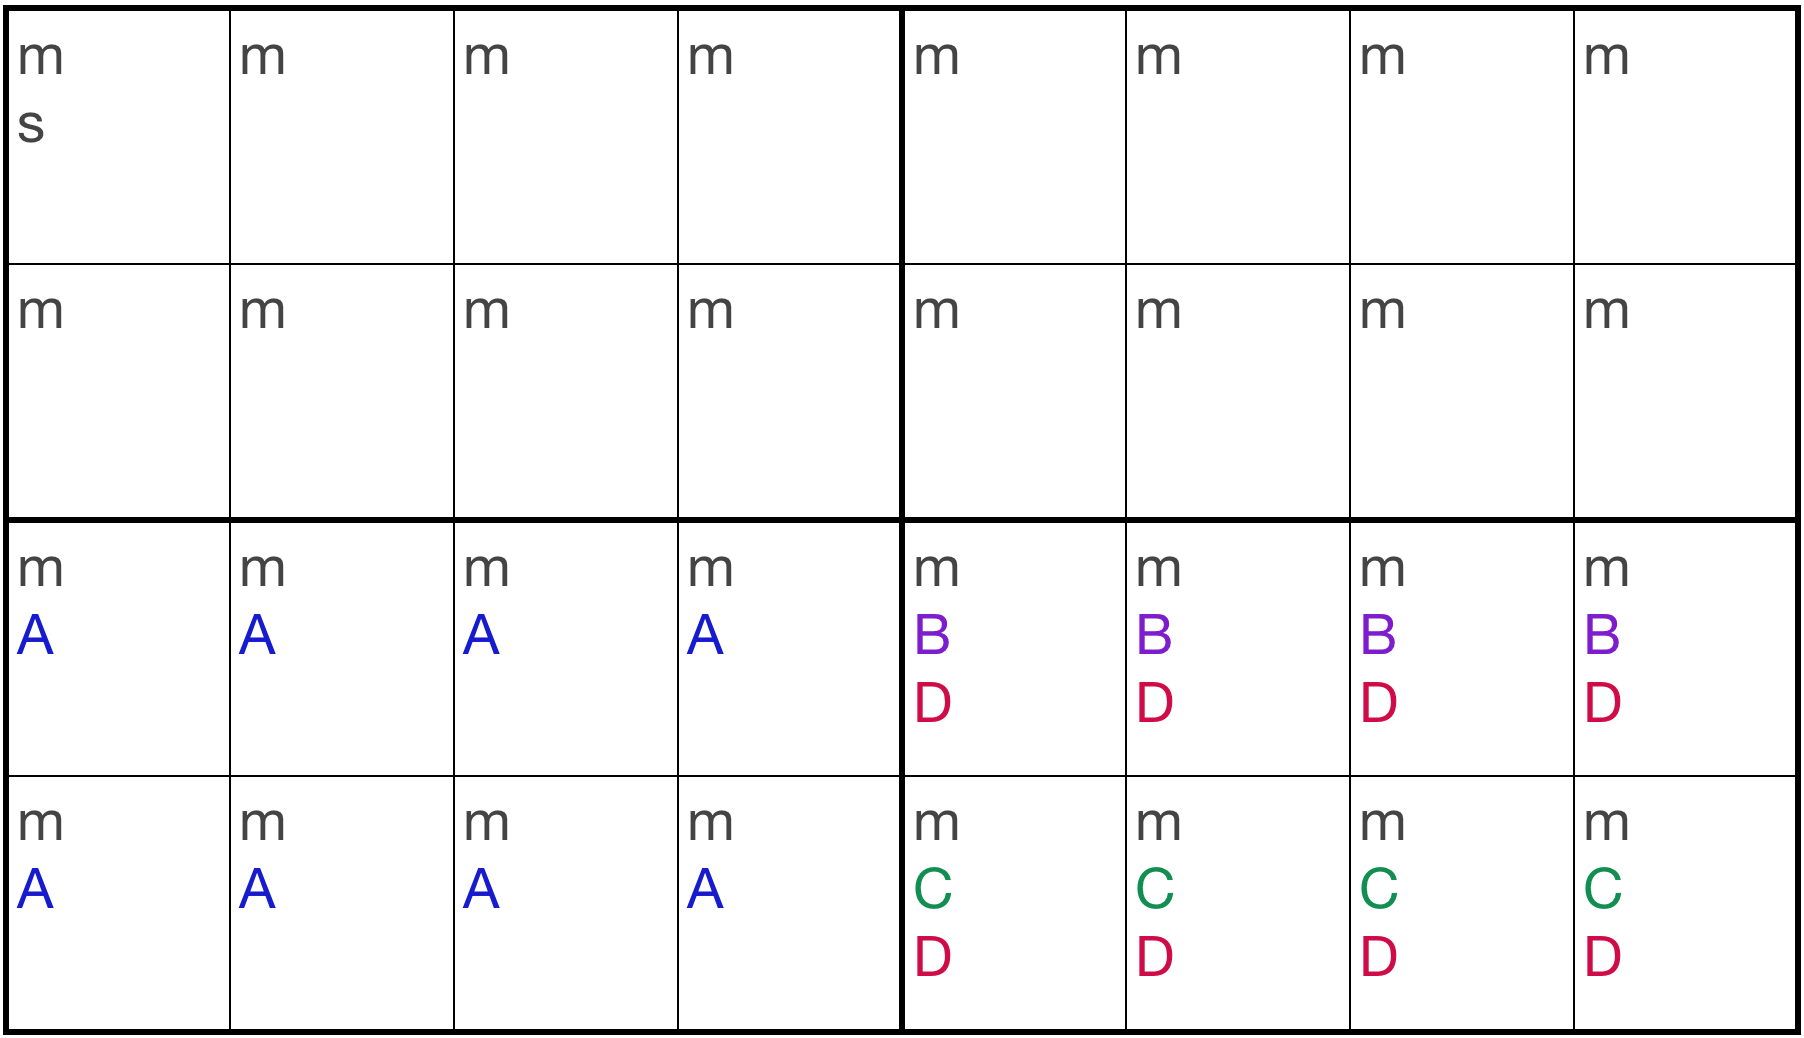
\includegraphics[width=\textwidth]{jm_example.png}
    \caption{An example 32-node layout, with four blocks of eight nodes.  Every node launches \jmmaster (m), one \jmscheduler (s) is spawned, and workers of different sizes (A, B, C, D) and requiring different resources are launched.  In this case, worker A consumes all the resources in a block, while B, C, and D can peacefully coexist in a block.  Perhaps D requires GPUs but only a few CPU cores, while B and C are CPU-intensive but do not need GPUs.}
    \label{fig:jm_example}
\end{figure}

\subsection{Masters}

\jmmaster is launched across the entire allocation with \mpirun (or equivalent), with one MPI task per node, as depicted in \figref{jm_example}.
Each \jmmaster also reports its location in the system hierarchy, so that they may be organized into blocks with fast communication, avoiding resource fragmentation across the communication fabric.

Workers can only be assigned resources inside a single block.  Each block gets a sub-communicator, through which the masters coordinate and launch workers.


\subsection{The Scheduler}

Just one instance of the scheduler is started, via \spawn (on the upper-left node in \figref{jm_example}).
It loads configuration information about the machine and assigns the masters to blocks with good communication performance.

After initialization, \jmscheduler begins to collect computational tasks, constructing a queue of work.
Each task knows a1

It matches work with available resources, performs a task-specific callback, dispatches them to the relevant block subcommunicator's rank-0 process, which starts the job via \spawn.
When the task is complete and the resources are marked free, another task-specific callback is made, so that logging, clean-up, or even the creation of new computational tasks can be accomplished.


\subsection{Workers}

Workers require minimal source modification.
One must include a single header, \texttt{jm.h}.
After the \mpiinit of a user application, one adds \jmhandshake, a handshake that reports to the local master and disconnects the communicator from the parent which launched it via \spawn.
One also adds \jmfinish just before \mpifinalize, allowing the worker to communicate its exit status and other information to its local master.

When workers are launched by the master via \spawn, they perform said handshake and reporting.
When workers are launched independently, they skip those steps, enabling the same binary to be launched in both ways.
This flexibility makes \mpijm-enabled applications easy to maintain, while also ensuring the same binary is executed during debugging as is executed during production.

Only if the worker crashes between launching and the disconnect of the intercommunicator can a problem in a worker (such as a call to \mpiabort) bring down the whole job.
Most executables perform only minimal work (such as simple initialization, reading of input files, etc.) between launching and the MPI initialization, providing very little opportunity for this to become an issue.
 

\subsection{Issues and Dependencies}

As it happens, many MPI implementations do not currently respect the specification, and the \spawn parent may abort if its child aborts, even after disconnection.\footnote{Bug reports are in the works, and we are exploring alternate architecture using other aspects of the MPI specification.}

The SpectrumMPI installed on the CORAL systems\footnote{(as of the beginning of May, 2018)} do not yet support \spawn, and other MPI libraries are not as highly optimized for these systems, yielding a $\sim$20\% performance hit in our initial tests.
We hope to have \spawn incorporated in the acceptance regimen for Summit at Oak Ridge.

\mpijm also depends on a \python installation, as will be discussed in \secref{python}.
